\subsubsection{TIMELY has no fixed point, is inherently unstable with
unpredictable fairness} 
A primary application of fluid models is to perform control theoretic analysis
on them. Similar to the analysis we performed for DCQCN in the previous section,
we attempted to perform the same analysis for TIMELY. The first step in
performing the analysis is to obtain the fixed point of the system, so we can
linearize the model about the fixed point and perform classical frequency domain
analysis. However, the way the TIMELY algorithm is implemented, it has \emph{no
fixed point}. The implication is that the queue length never converges, nor do
the sending rates of the flows. The system operates in limit cycles, always
oscillating. Moreover, while the system is oscillating, there are
\emph{infinite} solutions for the sending rates of the flows that satisfy the
fluid equations at any point. So, even if we can limit the magnitude of the
limit cycles by choosing parameters carefully, we can make no claims on the
fairness of the protocol since the system could be operating at any of those
infinite solutions. We first show that it has no fixed point.

\para{No fixed point for TIMELY:} 
In fixed point analysis, we identify the point at which the derivatives of the
various quantities in the fluid model become 0.  Setting $\tfrac{dq}{dt} = 0$,
we obtain $\sum_{i} R_i(t) = C$. Next, we have two possibilities, either $g > 0$
or $g  \le 0$. If $g$ takes a non-zero value, then $\tfrac{dg}{dt}$ cannot be 0,
as the second term in Equation~\ref{eq:timely_g} needs to be 0 for
$\tfrac{dq}{dt}$ to be 0. Thus, we require $g$ to be 0 at the fixed point.
However, from Equation~\ref{eq:timely_r}, we see that if $g = 0$,
$\tfrac{dR_i}{dt}$ \emph{cannot} be 0 since $\delta$ is not 0. Thus, from the
protocol description, the fluid model has no fixed points as the derivatives
cannot be simultaneously 0 and thus the (fluid) system never stabilizes to any
value. We modify the fluid model very slightly, by moving the equality condition
to the term involving $g$, and have a modified fluid model that looks like the
following:

\begin{equation}
\small
\frac{{dR_i}}{{dt}} = \left\{ \begin{array}{ll}
\frac{\delta }{{\tau *}}, & q(t - \tau ') < C*{T_{low}}\\
\frac{\delta }{{\tau *}}, & g < 0\\
 - \frac{{g\beta }}{{\tau *}}R(t), & g \ge 0\\
 - \frac{\beta }{{\tau *}}(1 - \frac{{C*{T_{high}}}}{{q(t - \tau ')}})R(t), & q(t - \tau ') > C*{T_{high}}
\end{array} \right.\\
\label{eq:timely_r_modified}
\end{equation}

\begin{figure*}[t]
\center
\subfigure[Both flows start at time 0 at 5Gbps] { 
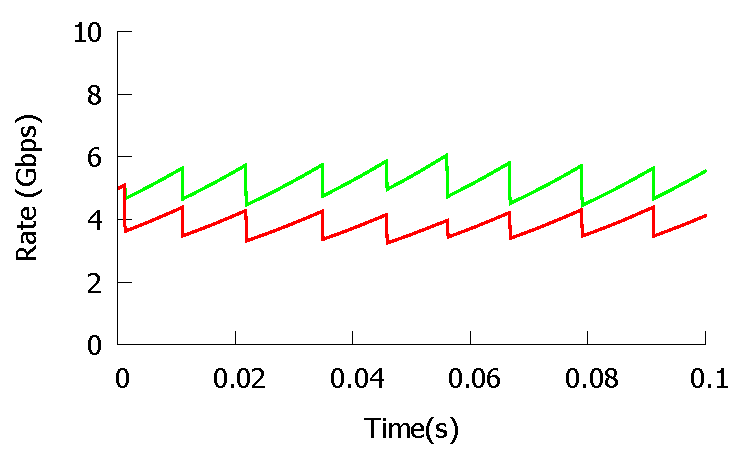
\includegraphics[width=0.3\textwidth]{figures/timely_stability_2f55.pdf}
}
\subfigure[Both start at 10Gbps, one starts 10ms late] { 
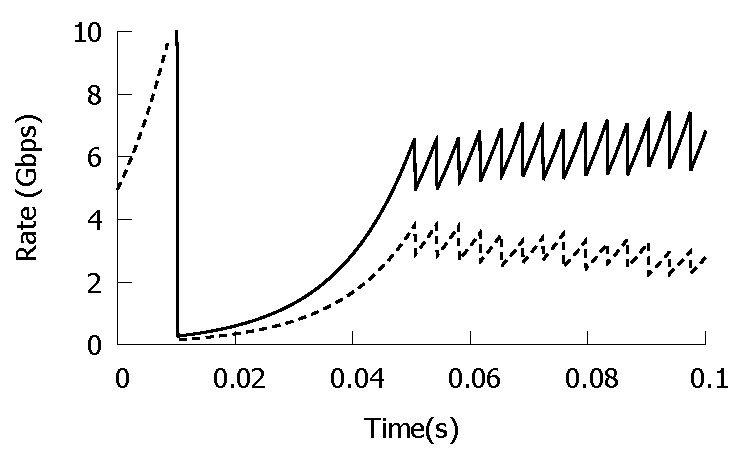
\includegraphics[width=0.3\textwidth]{figures/timely_stability_2ftime.pdf}
}
\subfigure[Both start at time 0, one at 7Gbps, other at 3Gbps] { 
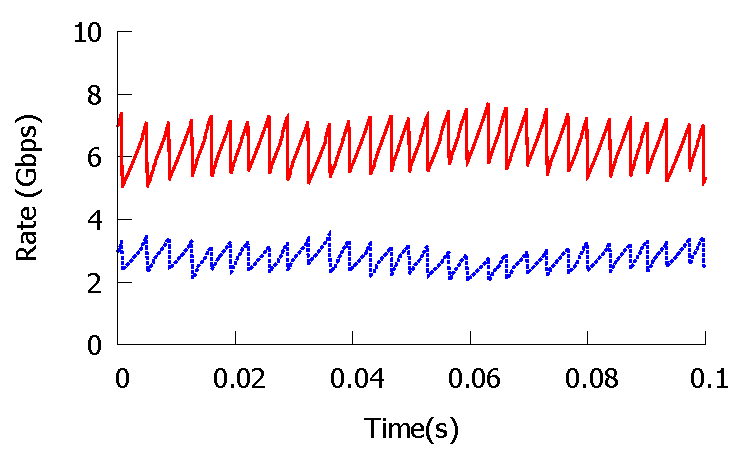
\includegraphics[width=0.3\textwidth]{figures/timely_stability_2f73.pdf}
}
\caption{Performance of two TIMELY flows under different starting conditions}
\label{fig:timely_unstable}
\end{figure*}

\para{Infinite fixed points for modified model:}
Practically, this change does not make much of a difference. With this
modification, we can now obtain the condition that with $g =0$, $\tfrac{dq}{dt}
= 0$, $\tfrac{dg}{dt} = 0$ and $C*T_{low} < q < C*T_{high}$. However, now we run
into the issue that TIMELY moves from zero fixed points to \emph{infinite} fixed
points. This is because to obtain $\tfrac{dg}{dt} =0$, we need $g = 0$ and
$\tfrac{dq}{dt} = 0$. Any value of $q$ between $C*T_{low} < q < C*T_{high}$
satisfies the condition and hence $q$ has infinitely many fixed points. As a
practical matter, those values are in fact finitely many and we can live with
the fact that $q$ will remain between $C*T_{low}$ and $C*T_{high}$. What is more
troubling is Equation~\ref{eq:timely_q}. According to that equation, at the
fixed point $\tfrac{dq}{dt} = 0$ as long as $\sum_{i} R(t) =  C$. From
Equation~\ref{eq:timely_r_modified}, we know that as long as $q$ is between the
thresholds and $g=0$, $\tfrac{dR_i}{dt} = 0$. Thus, the individual rates can
take on \emph{any} value, as long as they sum up to $C$ and we obtain the fixed
point. There is no requirement that at the fixed point $R_i = \tfrac{C}{N}$. In
fact, $\tfrac{R_{i}}{R_{j}}, i \ne j$ is not even bounded, so we cannot make any
claims on the fairness of TIMELY. Thus the fixed point of TIMELY is entirely
unpredictable and this is a fundamental flaw of the protocol. This is borne out
by the simulation results shown in Figure~\ref{fig:timely_unstable}, where we
only change the start time and initial rates of two flows, keeping everything
else constant, and we end up in completely different operating regimes.


%%% Local Variables:
%%% mode: latex
%%% TeX-master: "main"
%%% End:
